%%%%%%%%%%%%%%%%%%%%%%%%%%%%%%%%%%%%%%%%%%%%%%%%%%%%%%%%%%%%%%%%%%
%%This presentation was fullly copied from the WSC presentation (dec. 2015)
%% and addapted for the CAA2k16
%% and then  for the EPNET workshop of the 3rd of may
%% and then  for the SM7 workshop of the  of may
\documentclass[12pt, notes=show]{beamer}
\usetheme[width=0cm]{Goettingen}
\usecolortheme{rose}
\useoutertheme{default}
\setbeamerfont{caption}{size=\scriptsize}
\setbeamertemplate{navigation symbols}{}

\addtobeamertemplate{navigation symbols}{}{%
	\usebeamerfont{footline}%
	\usebeamercolor[fg]{footline}%
	\hspace{1em}%
	$\dfrac{\insertframenumber}{\inserttotalframenumber}$
}

\usepackage{color} 
\usepackage{tikz} 
\usepackage{fontspec} 
\usepackage{array}
\setsansfont{Futura LT}

\definecolor{siris}{HTML}{1C0E66} 

\title{Computer modelling and simulation as heuristic tool to understand the past: the case of the EPNEt project.}
\author{Simon Carrignon, Alessandro Mosca, Bernardo Rondelli \& José Remesal}

\institute{19 May 2016}


\date{
	\scriptsize
	\begin{columns}
		\begin{column}{.3\textwidth}
			\begin{center}
				\includegraphics[height=1cm]{images/bscLogo.jpg} 
			\end{center}
		\end{column}

		\begin{column}{.3\textwidth}
		    \begin{center}
			\includegraphics[height=1cm]{images/UB_logo.png}\\

			\colorbox{siris}{\centering
			    \includegraphics[height=.8cm]{images/siris_logo_menu1.png} }
			\end{center}
		\end{column}

		\begin{column}{.3\textwidth}
			\begin{center}
				\includegraphics[height=1cm]{images/upfLogo.jpeg}
			\end{center}
		\end{column}
	\end{columns}

}

\begin{document}
\begin{frame}
    \maketitle
\end{frame}

\begin{frame}{Introduction}
   \begin{enumerate}
       \item Evolutionary Biology
       \item History \&  Archaeology
       \item Interdisciplinary
   \end{enumerate}

%Incompleteness and uncertainty of the historical and archaeological record affect historical interpretation \cite{madella2014}. In this paper, we argue that \emph{formal modelling} and computer Simulation are valuable tools to overcome such limitations. We first show how evolutionary biologists have successfully embraced these tools and why their epistemological framework is close to what archaeologists and historians do. We then defend how those M\&S are good heuristic tools in science in general and we finished by introducing an interdisciplinary research setting, where the previous points can be exploited in a meaningful way to investigate historical questions.
\end{frame}

\begin{frame}
    \begin{center}
	\Huge
	Computer Simulation \\ applied to\\ 
	Evolutionary Biology
    \end{center}
\end{frame}
%\begin{frame}{Evolutionary Biology}
%The goal of evolutionary biologists is to understand the mechanisms at the origin of the living world as we can observe it. Assuming the theory of evolution, they characterise the succession of past events that constitute this story. Starting with Gould \cite{gould1989wonderfullife}, several biologists and philosophers have argued that the nature of this research activity is historical \cite{beatty1995evolutionary}: the actual biological world does not depend \emph{only} on biological rules, but on the uniqueness of the succession of events. To encompass the issues raised by such historicity, evolutionary biologists use, at least since the Modern Synthesis, formal models to figure out different possible successions of events and the likelihood of such possible historical paths, and they test it against the available data.
%\end{frame}

\begin{frame}{Evolutionary Biology}
Succession of events $\rightarrow$ Actual Biology?
	\begin{center}
	    \includegraphics[width=.8\textheight]{images/treeOfLife.png}
	\end{center}
\end{frame}
\begin{frame}{Unusual Scientific Task}
    %Darwin theory (Gayon, 1992)
    \vfill
    \begin{itemize}
	\item Difficult to prove
	    \vfill
	\item No absolute values (Statistics \& Probabilities)
	    \vfill
	\item  Highly path dependent (Gould Wonderful Life , Beatty Contingency thesis)
    \end{itemize}
    \vfill
\end{frame}


\begin{frame}{Evolutionary biology toolkit} 
	\begin{itemize}
		\item<1-> Since the biometricians:\\
			Detecting Pattern\\
			\uncover<2->{\begin{figure}
				\includegraphics[width=.5\textwidth]{images/weldon.png}
				\caption{Weldon \& Pearson 1892}
			\end{figure}
		}
			
			
		\item<3-> Mathematical models of idealized situation:\\
		    {\small Hardy Weinberg, Fisher-Wrights models, Lotka-Volterra equations\ldots}
		\item<4->Complexity $\uparrow$ quickly. 
	\end{itemize}
\end{frame}

\begin{frame}{Computer Simulation}
    \begin{itemize}
	\item<1-> Simulate mathematical model (Bayesian inference \& model selection)
	\item<4-> Focus on complex interactions (Evolutionary Ecology, EvoDevo\dots)
	\item<7-> \dots
    \end{itemize}
    
    \begin{table}
	\centering
	\begin{tabular}{ccc}
	    \uncover<2->{ \includegraphics[height=2.5cm]{images/baeysPhilo.jpg} }& \uncover<6->{\includegraphics[height=2.5cm]{images/abmEco.png}}&
	    \uncover<3->{\includegraphics[height=2.5cm]{images/baeysEvol.jpg}}\\ 
	    \uncover<8->{\includegraphics[height=2.5cm]{images/netlogo.jpg}}&\uncover<5->{\includegraphics[height=2.5cm]{images/computerSimulation.jpg}} &\uncover<9->{\includegraphics[height=2.5cm]{images/insilico.jpg}}\\
	\end{tabular}
    \end{table}
    
\end{frame}


%\begin{frame}
%    \centering\Huge
%    Computer Model \& Simulation
%\end{frame}
%\begin{frame}{Alife Classification}
%   Barandiaran~et~al.~2006 propose 4 class of epistemic models:
%	\begin{enumerate}
%    \vfill
%	    \item <2-> Generic:\\
%		\uncover<3->{\small \hspace{.5cm} General model equivalent to mathematical description (scale free network)}
%	    \vfill
%	    \item <4-> Conceptual: \\
%		\uncover<5->{\small \hspace{.5cm} To explore theoretical assumption and concepts (Baldwin effect) }
%	    \vfill
%	    \item <6-> Functional: \\
%		\uncover<7->{\small \hspace{.5cm} To understand (unknown) causal processes underlying emergent properties (ant foraging model)} 
%	    \vfill
%	    \item <8-> Mechanistic: \\
%		\uncover<9->{\small \hspace{.5cm} One to One correspond with natural system (Model of bacterial chemotaxis)}
%	\end{enumerate}
%	    \vfill
%\end{frame}
%
%\begin{frame}{General Advantages}
%
%    \vfill
%	Conceptual Models has Opaque Thought Experiment (Paolo~et~al.~2000)
%    \vfill
%	\begin{itemize}
%    \vfill
%	    \item <2-> Thought Experiment:\\
%		\uncover<3->{\small \hspace{.5cm} Higher degree of freedom than experimental methods ()}
%	    \vfill
%	    \item <4-> Experiment: \\
%		\uncover<5->{\small \hspace{.5cm} Higher degree of de-idealization than theory or though experiments}
%	    \vfill
%	    \item <6-> Opacity: \\
%		\uncover<7->{\small \hspace{.5cm}  Experiment \emph{per se}}
%	\end{itemize}
%	    \vfill
%%%This use of computer simulations and modelling is not restricted to evolutionary biology. It is now widely spread in all branches of Science. People in artificial life \cite{paolo00simulationmodelsasopaquethoughtexperiments} argue that computer simulation are powerful heuristic tools that combine the exploratory power of thought experiments and the logical strength of mathematics. They allow to test quickly a lot of possible ``opaque though experiments'' that would be impossible to execute mentally. Moreover, in complex systems where the interactions of every subcomponents are multiple, the global dynamics are difficult to predict analytically, which make simulation and modelling one of the best suitable tool to explore and study those mechanisms.
%\end{frame}
%

\begin{frame}
    \begin{center}
	\Huge
	Computer Simulation \\ applied to\\  History \& Archaeology
    \end{center}
\end{frame}


\begin{frame}{History}

    \uncover<2->{Understand succession of events that led to nowadays human societies:}
    \begin{itemize}
	\item <3-> Highly Path Depend
	\item <4-> Non absolute value
    \end{itemize}
    
\end{frame}

\begin{frame}{History}
%This suggest that (i) the problems encountered by evolutionary biologists are close to those archaeologists and historians have to face (ii) the way inferences are made about the history of living beings and the history of human societies fall into a similar epistemological framework and (iii) mathematical and computer models are good candidates to infer, in a statistically plausible and transparent way, missing data and complex hypotheses in both enterprise.
    Nonetheless:
    \begin{itemize}
	\item<2-> Hypothesis rarely formalized and quantifiable, 
	\item<3-> Empirical experimentation less accessible,
	\item<4-> Higher level of complexity:
    \end{itemize}
\end{frame}

\begin{frame}{History}
    \begin{columns}
	\begin{column}{.4\textwidth}
	    \begin{center}
		\uncover<2->{Hybridization of peas\\
		    \includegraphics[width=.5\textwidth]{images/peas.jpg}
		
		}
		\uncover<3->{
		    \includegraphics[height=1.5cm]{images/MendelExpe.png}

		}
		\uncover<4->{$\downarrow$}

		\uncover<5->{
		    \includegraphics[height=3.5cm]{images/MendelShema.jpg}\\
		    {\tiny(Mendel's principles)}
		}

	    \end{center}
	\end{column}
	\begin{column}{.5\textwidth}
	    \begin{center}
		\uncover<6->{City Growth\\}
		\vspace{.5cm}
		\uncover<7->{
		    \includegraphics[height=2cm]{images/santCugat1946.png} \hspace{.5cm} 
		    \includegraphics[height=2cm]{images/santCugat2014.png} \\ 
{\tiny(Sant Cugat 1946)} \hspace{.5cm} 
{ \tiny(Sant Cugat 2014)}\\
		}
		\vspace{1cm}
		\uncover<8->{$\downarrow$}
		\vspace{1cm}

		\uncover<9->{
		    {\Huge ?}
		}
		\vspace{1cm}

	\end{center}
	    \end{column}
    \end{columns}
	

\end{frame}

\begin{frame}{Computer Simulation}

    \begin{columns}
	\begin{column}{.4\textwidth}
	    \begin{center}
		\uncover<2->{
		    \includegraphics[height=2cm]{images/simcityStart.png} \\ 
		}
		\uncover<3->{
		    \includegraphics[height=2cm]{images/simcityStart.png} \\ 
		}
		\uncover<4->{
		    \dots \\ 
		    \vspace{.5cm}
		}
		\uncover<5->{
		    \includegraphics[height=2cm]{images/simcityStart.png} \\ 
		}

	    \end{center}
	\end{column}
	\begin{column}{.2\textwidth}
	    \uncover<6->{
		$\rightarrow$
	    }
	    
	\end{column}
	\begin{column}{.4\textwidth}
	    \uncover<7->{
		\includegraphics[height=2cm]{images/simCityEnd2} \\
		    \vspace{.5cm}
	    }
	    \uncover<8->{
		\includegraphics[height=2cm]{images/simCityEnd.png} 
	    }
	    
	    
	\end{column}
    \end{columns}
	
\end{frame}



\begin{frame}{Historical Hypothesis: Quantitative analysis}
    Rubio-Campillo 2015:  Model of War casualties
    \begin{itemize}
	\item<1-> Formalized hypothesis 
	\item<2-> Available data
    \end{itemize}

    \uncover<3->{Different hypothesis to explain historical patterns}
    \begin{center}
	\uncover<4->{\includegraphics[width=.8\textwidth]{images/armyCasualties.png} }
    \end{center}


\end{frame}

\begin{frame}{Quantitative analysis}
    4 models to explain Battle Casualties
    \begin{itemize}
	\item<5->Compare and select the best Hypothesis.
    \end{itemize}
    \begin{enumerate}
	\item<1->Linear 
	\item<2->Squared 
	\item<3->Logarithmic
	\item<4->Fatigue
    \end{enumerate}
    

    \begin{table}
	\begin{tabular}{cccc}
	    \uncover<1->{\includegraphics[width=2cm]{images/linEq}}&
	    \uncover<2->{\includegraphics[width=2cm]{images/squEq}}&
	    \uncover<3->{\includegraphics[width=2cm]{images/logEq}}&
	    \uncover<4->{\includegraphics[width=2cm]{images/fatEq}}\\
	    \uncover<5->{Let P ratio r/b = 1.5}\\
	    \uncover<6->{\includegraphics[width=2cm]{images/linGra}}&
	    \uncover<7->{\includegraphics[width=2cm]{images/squGra}}&
	    \uncover<8->{\includegraphics[width=2cm]{images/logGra}}&
	    \uncover<9->{\includegraphics[width=2cm]{images/fatGra}}\\
	\end{tabular}
    \end{table}
\end{frame}

\begin{frame}{Quantitative analysis}
    \begin{columns}
	\begin{column}{.6\textwidth}
	    \begin{center}
		\includegraphics[width=\textwidth]{images/resultXavi.png} 
	    \end{center}
	\end{column}
	\begin{column}{.45\textwidth}
	    Fatigue model outperform all
	\end{column}
    \end{columns}
    Computer Simulation
	\begin{enumerate}
	    \item<2-> Paliate lack of empirical data and difficulty to gather new
	    \item<3-> Statistical validation of hypothesis
	\end{enumerate}
\end{frame}



\begin{frame}{Formal Description \& Comparison}
    \begin{columns}
	\begin{column}{.6\textwidth}
	    \begin{center}
		\includegraphics[width=\textwidth]{images/wareRome.png} 
	    \end{center}
	\end{column}
	\begin{column}{.45\textwidth}
	\small Brughman \& Poblome 2016: Nature of the Market
	\end{column}
    \end{columns}
	\begin{enumerate}
	    \item<2-> Loosely formalised or complex Hypothesis
	    \item<3-> Heterogeneous Data and Knowledge
	\end{enumerate}

	\uncover<4->{Model to:}
	\begin{itemize}
	    \item<5-> Formally describe the hypotheses
	    \item<6-> Quantitatively compare it
	\end{itemize}

\end{frame}

\begin{frame}{Formal Description \& Comparison}
	\only<1>{
	    Hypothesis:
	    
	    \begin{columns}
		\begin{column}{.4\textwidth}
		    \begin{center}
			\includegraphics[height=6cm]{images/bazaarBang.jpg}\\
			Independent Markets

		    \end{center}
		\end{column}
		\begin{column}{.4\textwidth}
		    \begin{center}
			\includegraphics[height=6cm]{images/marketTemin.jpg}\\
			Integrate Market

		    \end{center}
		\end{column}
	    \end{columns}
	}
	\only<2>{
	    Formalisation:
	    \begin{center}
		\begin{columns}
		    \begin{column}{.4\textwidth}
			\includegraphics[height=4cm]{images/marketIntegration.png}\\

		    \end{column}
		    \begin{column}{.4\textwidth}

		\includegraphics[height=6cm]{images/formalModel.png}
		    \end{column}
		\end{columns}
	    \end{center}
    }

\end{frame}
\begin{frame}{Formal Description \& Comparison}
	Result:\\
	\begin{center}

	    \only<1>{		    \includegraphics[height=6cm]{images/looselyMarket.png}\\ Independant Market}
	    \only<2>{		    \includegraphics[height=6cm]{images/highMarket.png}\\ Integrated Market}
	\end{center}

\end{frame}


\begin{frame}{Hypothesis Generation}
\end{frame}



\begin{frame}{Cultural Transmission}
    \begin{columns}
	\begin{column}{.6\textwidth}
	    \includegraphics[width=.9\textwidth]{images/Beti.png}
	\end{column}
	\begin{column}{.3\textwidth}
	     \includegraphics<2->[width=.9\textwidth]{images/mesures.png}
	\end{column}
    \end{columns}

    \uncover<3->{
	Cultural transmission of manufacturings techniques:
    \begin{itemize}
	\item Few Data
	\item Few Hypothesis 
    \end{itemize}
}
\end{frame}


\begin{frame}{Hypothesis Generation}
	\includegraphics[height=6cm]{images/pca.png}
\end{frame}


\begin{frame}{Hypothesis Generation}
    
    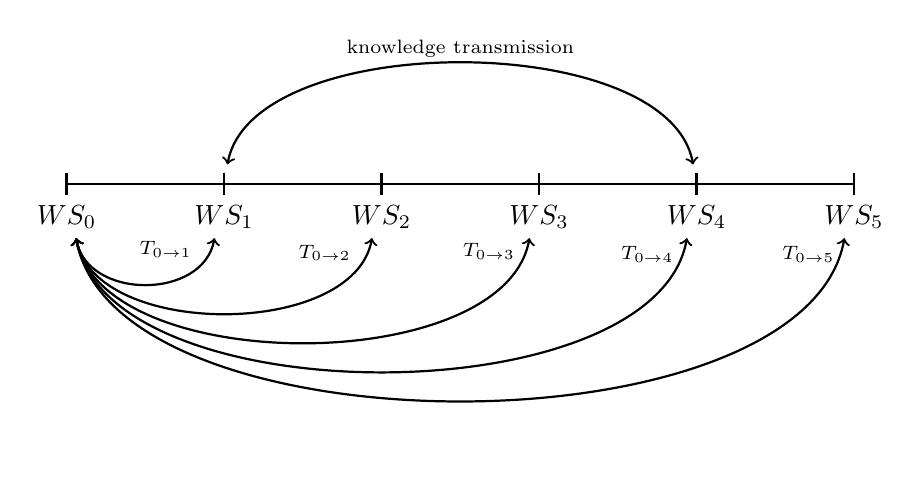
\begin{tikzpicture}[thick,scale=2]
	\coordinate (WS0) at (0,0);
	\coordinate (WS1) at (1,0);
	\coordinate (WS2) at (2,0);
	\coordinate (WS3) at (3,0);
	\coordinate (WS4) at (4,0);
	\coordinate (WS5) at (5,0);

	\draw[thick,-] (0,0) -- (5,0) node[anchor=north west] {};   
	\foreach \x in {0,1,2,3,4,5}
	\draw (\x cm,2pt) -- (\x cm,-2pt) node[anchor=north] {$WS_\x$};


	\uncover<2->{	\draw [black,shorten <= 0.25cm, shorten >= 0.25cm, <->] (WS1) to[out=80,in=100,distance=1cm] node[above,font=\scriptsize]{knowledge transmission} (WS4); }


	\uncover<3->{\draw [black,shorten <= 0.7cm, shorten >= 0.7cm, <->] (WS0) to[out=-80,in=-100,distance=.75cm	]  node[font=\scriptsize,pos=.60	,above]{$T_{0 \rightarrow 1}$} (WS1);}
	\uncover<4->{\draw [black,shorten <= 0.7cm, shorten >= 0.7cm, <->] (WS0) to[out=-80,in=-100,distance=1cm	]  node[font=\scriptsize,pos=.75	,above]{$T_{0 \rightarrow 2}$}(WS2);}
	\uncover<5->{\draw [black,shorten <= 0.7cm, shorten >= 0.7cm, <->] (WS0) to[out=-80,in=-100,distance=1.25cm	]  node[font=\scriptsize,pos=.82		,above]{$T_{0 \rightarrow 3}$}(WS3);}
	\uncover<6->{\draw [black,shorten <= 0.7cm, shorten >= 0.7cm, <->] (WS0) to[out=-80,in=-100,distance=1.5cm	]  node[font=\scriptsize,pos=.85	,above]{$T_{0 \rightarrow 4}$}(WS4);}
	\uncover<7->{\draw [black,shorten <= 0.7cm, shorten >= 0.7cm, <->] (WS0) to[out=-80,in=-100,distance=1.75cm	]  node[font=\scriptsize,pos=.875	,above]{$T_{0 \rightarrow 5}$}(WS5);}

    \end{tikzpicture}

    \uncover<8->{

	\begin{itemize}
	    \item<8-> $T_{A\rightarrow B}$ the transmission of information between A \& B:
	    \item<9-> $P(T_{A\rightarrow B})$ and $P(T_{A\rightarrow B})>P(T_{A\rightarrow C})$ if $|A-B|<|A-C|$
	\end{itemize}
    }

\end{frame}

\begin{frame}{Result}
    \begin{tabular}{m{5cm}m{5cm}}
	    %&No Transmission & Transmission \\\hline

	\resizebox{5cm}{!}{
	    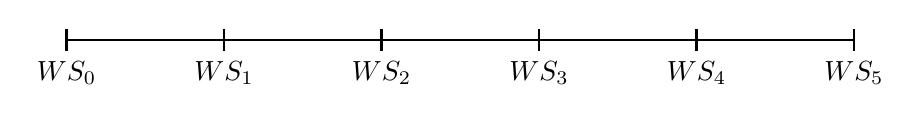
\begin{tikzpicture}[thick,scale=2]
		\coordinate (WS0) at (0,0);
		\coordinate (WS1) at (1,0);
		\coordinate (WS2) at (2,0);
		\coordinate (WS3) at (3,0);
		\coordinate (WS4) at (4,0);
		\coordinate (WS5) at (5,0);
		\draw[thick,-] (0,0) -- (5,0) node[anchor=north west] {};   
		\foreach \x in {0,1,2,3,4,5}
		\draw (\x cm,2pt) -- (\x cm,-2pt) node[anchor=north] {$WS_\x$};

	    \end{tikzpicture}
	}
	&

	\resizebox{5cm}{!}{
	    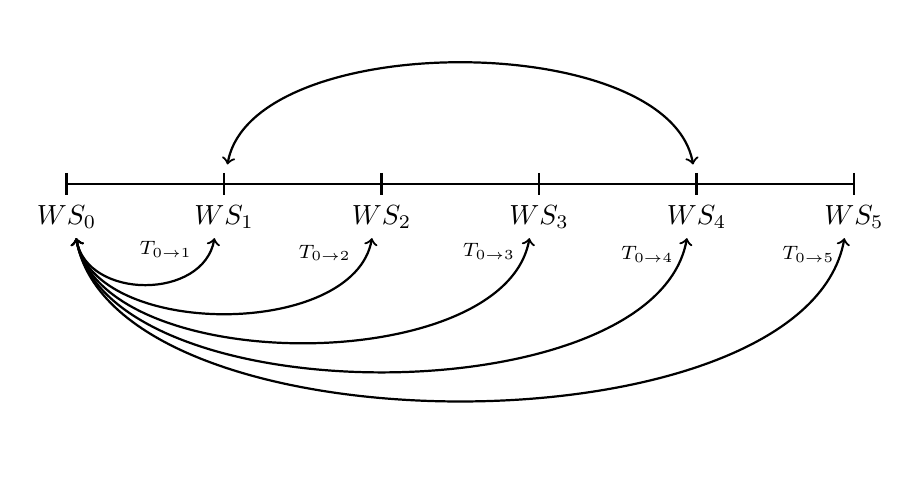
\begin{tikzpicture}[thick,scale=2]
		\coordinate (WS0) at (0,0);
		\coordinate (WS1) at (1,0);
		\coordinate (WS2) at (2,0);
		\coordinate (WS3) at (3,0);
		\coordinate (WS4) at (4,0);
		\coordinate (WS5) at (5,0);
		\draw[thick,-] (0,0) -- (5,0) node[anchor=north west] {};   
		\foreach \x in {0,1,2,3,4,5}
		\draw (\x cm,2pt) -- (\x cm,-2pt) node[anchor=north] {$WS_\x$};

		\draw [black,shorten <= 0.25cm, shorten >= 0.25cm, <->] (WS1) to[out=80,in=100,distance=1cm] (WS4); 
		\draw [black,shorten <= 0.7cm, shorten >= 0.7cm, <->] (WS0) to[out=-80,in=-100,distance=.75cm	]  node[font=\scriptsize,pos=.60	,above]{$T_{0 \rightarrow 1}$}(WS1);
		\draw [black,shorten <= 0.7cm, shorten >= 0.7cm, <->] (WS0) to[out=-80,in=-100,distance=1cm	]  node[font=\scriptsize,pos=.75	,above]{$T_{0 \rightarrow 2}$}(WS2);
		\draw [black,shorten <= 0.7cm, shorten >= 0.7cm, <->] (WS0) to[out=-80,in=-100,distance=1.25cm	]  node[font=\scriptsize,pos=.82	,above]{$T_{0 \rightarrow 3}$}(WS3);
		\draw [black,shorten <= 0.7cm, shorten >= 0.7cm, <->] (WS0) to[out=-80,in=-100,distance=1.5cm	]  node[font=\scriptsize,pos=.85	,above]{$T_{0 \rightarrow 4}$}(WS4);
		\draw [black,shorten <= 0.7cm, shorten >= 0.7cm, <->] (WS0) to[out=-80,in=-100,distance=1.75cm	]  node[font=\scriptsize,pos=.875	,above]{$T_{0 \rightarrow 5}$}(WS5);
	    \end{tikzpicture}
	}
	\\
	\resizebox{5cm}{!}{
	    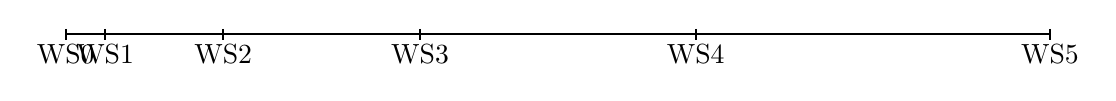
\begin{tikzpicture}[thick,scale=.5]
		\coordinate (WS0) at (0,0);
		\coordinate (WS1) at (1,0);
		\coordinate (WS2) at (4,0);
		\coordinate (WS3) at (9,0);
		\coordinate (WS4) at (16,0);
		\coordinate (WS5) at (25,0);
		\draw[thick,-] (0,0) -- (25,0) node[anchor=north west] {};   
		\foreach \x in {0,1,4,9,16,25}
		\draw (\x cm,4pt) -- (\x cm,-4pt) node[anchor=north] {};
		\draw (WS0) node[anchor=north]{WS0};
		\draw (WS1)node[anchor=north]{WS1};
		\draw (WS2)node[anchor=north]{WS2};
		\draw (WS3)node[anchor=north]{WS3};
		\draw (WS4)node[anchor=north]{WS4};
		\draw (WS5)node[anchor=north]{WS5};
	    \end{tikzpicture}
	}	&
	\resizebox{5cm}{!}{
	    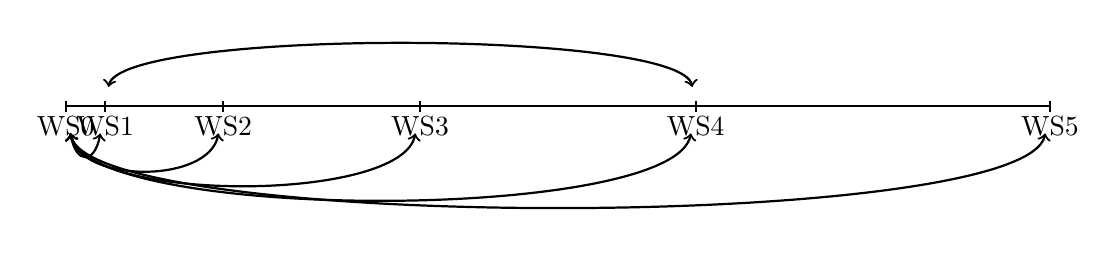
\begin{tikzpicture}[thick,scale=.5]
		\coordinate (WS0) at (0,0);
		\coordinate (WS1) at (1,0);
		\coordinate (WS2) at (4,0);
		\coordinate (WS3) at (9,0);
		\coordinate (WS4) at (16,0);
		\coordinate (WS5) at (25,0);
		\draw[thick,-] (0,0) -- (25,0) node[anchor=north west] {};   
		\foreach \x in {0,1,4,9,16,25}
		\draw (\x cm,4pt) -- (\x cm,-4pt) node[anchor=north] {};
		\draw (WS0) node[anchor=north]{WS0};
		\draw (WS1)node[anchor=north]{WS1};
		\draw (WS2)node[anchor=north]{WS2};
		\draw (WS3)node[anchor=north]{WS3};
		\draw (WS4)node[anchor=north]{WS4};
		\draw (WS5)node[anchor=north]{WS5};

		\draw [black,shorten <= 0.25cm, shorten >= 0.25cm, <->] (WS1) to[out=80,in=100,distance=2cm] (WS4); 
		\draw [black,shorten <= .35cm, shorten >= .35cm, <->] (WS0) to[out=-80,in=-100,distance=1.5cm	]  (WS1);
		\draw [black,shorten <= .35cm, shorten >= .35cm, <->] (WS0) to[out=-80,in=-100,distance=2cm	]  (WS2);
		\draw [black,shorten <= .35cm, shorten >= .35cm, <->] (WS0) to[out=-80,in=-100,distance=2.5cm	]  (WS3);
		\draw [black,shorten <= .35cm, shorten >= .35cm, <->] (WS0) to[out=-80,in=-100,distance=3cm	]  (WS4);
		\draw [black,shorten <= .35cm, shorten >= .35cm, <->] (WS0) to[out=-80,in=-100,distance=3.25cm	]  (WS5);
	    \end{tikzpicture}
	}	\\

    \end{tabular}

\end{frame}

\begin{frame}{Hypothesis Generation}
    
    Explore hypothetics situation, generate and compare hopthesis :\\
    \hspace{.5cm}Conceptual Model (Barandian 2006) as Opaque thought experiement (Di Paolo 2000).

\end{frame}

\begin{frame}{Model in History}
    \begin{itemize}
	\item Not exhaustive list
	\item Not fixed status
	\item Help at different level

    \end{itemize}
    

\end{frame}

\begin{frame}{Limitation}
    Assumptions made at every level, complex interpretation:\\
    \hfil $\rightarrow$ Need of multi-disciplinarity
%However, building computational simulations that can provide valuable knowledge about the modelled object still remains a difficult task. Computer scientists have to be aware of every assumptions they could implicitly made and domain experts (as historians or biologists) have to formulate their hypotheses in an epistemological framework yet not clearly specified and far from the one they are used. The communication is thus primordial: knowledge here does not lie in the mathematical models neither in the historical data but emerges from the well articulation of both side \cite{winsberg09taletwomethods}.
\end{frame}

\begin{frame}
    \begin{center}
	\Huge
	Interdisciplinarity
    \end{center}
\end{frame}

\begin{frame}{Interdisciplinarity}
    Warren Weaver, 1948:
	\begin{center}
	    \includegraphics<1>[width=.8\textwidth]{images/inter0}
	    \includegraphics<2>[width=.8\textwidth]{images/inter1}
	    \includegraphics<3>[width=.8\textwidth]{images/inter2}
	    \includegraphics<4>[width=.8\textwidth]{images/inter3}
	\end{center}
%Here we provide examples from the EPNet project, where the emphasis is on supporting historians with computational infrastructure for understanding the political and economical implications behind food production and distribution along the Roman Empire. By taking into consideration the design and development of such a computational infrastructure, the EPNet epistemological framework is aiming to address three main problems: (i) structuring and making accessible large collections of data through the Web, (ii) providing a formally defined, unambiguous, framework for analysing the data and exporting them in a way that can be further manipulated by computer simulation algorithms, and complex network analysis, and (iii) making each collection of data integrable with other complementary data sources.
\end{frame}


\begin{frame}{Interdisciplinarity}
    \begin{center}
	\includegraphics<1>[width=.8\textwidth]{images/interdsiciplinarity0.png}
	\includegraphics<2>[width=.8\textwidth]{images/interdsiciplinarity1.png}
	\includegraphics<3>[width=.8\textwidth]{images/interdsiciplinarity2.png}
	\includegraphics<4>[width=.8\textwidth]{images/interdsiciplinarity3.png}
	\includegraphics<5>[width=.8\textwidth]{images/interdsiciplinarity4.png}
	\includegraphics<6>[width=.8\textwidth]{images/interdsiciplinarity5.png}
	\includegraphics<7>[width=.8\textwidth]{images/interdsiciplinarity6.png}
	\includegraphics<8>[width=.8\textwidth]{images/interdsiciplinarity.png}
    \end{center}
\end{frame}

\begin{frame}{EPNet Project}
\end{frame}

\end{document}

